\documentclass[tikz,border=8pt]{standalone}

\usepackage[T1]{fontenc}
\usepackage[utf8]{inputenc}
\usepackage{lmodern}
\usepackage{tikz}
\usetikzlibrary{arrows.meta,positioning,fit,calc,backgrounds}

\begin{document}
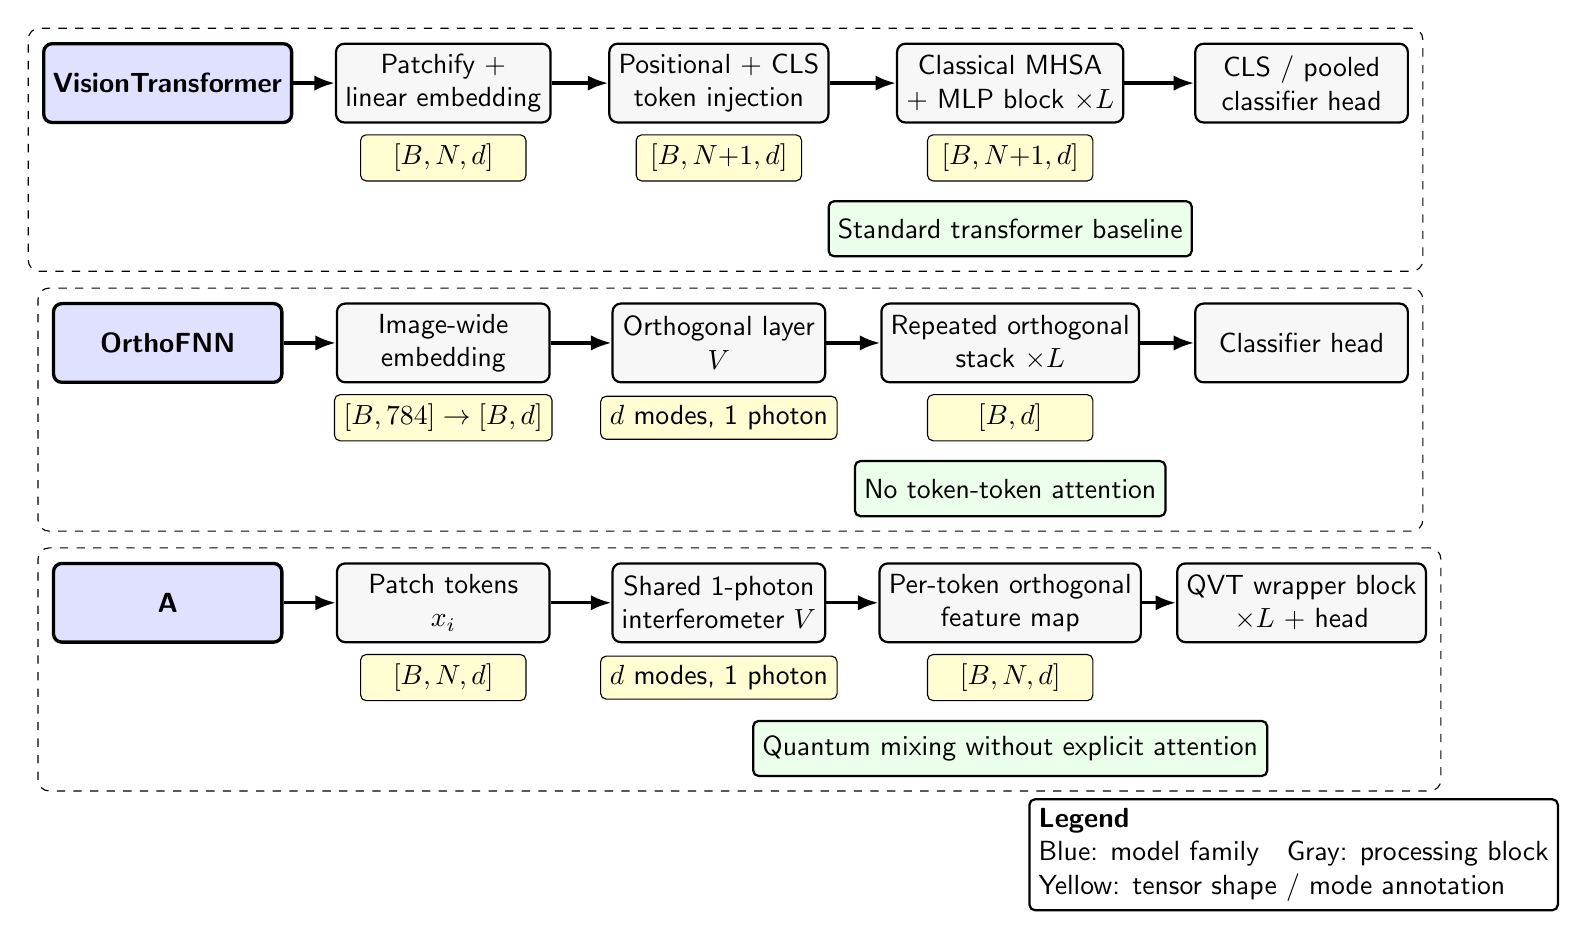
\begin{tikzpicture}[
  font=\sffamily,
  x=1cm, y=1cm,
  model/.style={draw, rounded corners=3pt, minimum width=2.9cm, minimum height=1cm, align=center, fill=blue!12, very thick},
  stage/.style={draw, rounded corners=3pt, minimum width=2.7cm, minimum height=1cm, align=center, fill=gray!6, thick},
  ann/.style={draw, rounded corners=2pt, minimum width=2.1cm, minimum height=0.5cm, align=center, fill=yellow!18, thin},
  note/.style={draw, rounded corners=2pt, minimum width=2.4cm, minimum height=0.7cm, align=center, fill=green!8, thick},
  legend/.style={draw, rounded corners=2pt, minimum width=4.5cm, minimum height=0.7cm, align=left, fill=white, thick},
  arrow/.style={-{Latex[length=2.6mm]}, very thick},
  dashedbox/.style={draw, dashed, rounded corners=4pt, inner sep=5pt}
]

\node[model] (vt) at (1.7, 0) {\textbf{VisionTransformer}};
\node[stage] (vt1) at (5.2, 0) {Patchify +\\linear embedding};
\node[stage] (vt2) at (8.7, 0) {Positional + CLS\\token injection};
\node[stage] (vt3) at (12.4, 0) {Classical MHSA\\+ MLP block $\times L$};
\node[stage] (vt4) at (16.1, 0) {CLS / pooled\\classifier head};
\node[ann] (vts1) at (5.2, -0.95) {$[B,N,d]$};
\node[ann] (vts2) at (8.7, -0.95) {$[B,N{+}1,d]$};
\node[ann] (vts3) at (12.4, -0.95) {$[B,N{+}1,d]$};
\node[note]  (vtn) at (12.4, -1.85) {Standard transformer baseline};

\node[model] (ofnn) at (1.7, -3.3) {\textbf{OrthoFNN}};
\node[stage] (of1) at (5.2, -3.3) {Image-wide\\embedding};
\node[stage] (of2) at (8.7, -3.3) {Orthogonal layer\\$V$};
\node[stage] (of3) at (12.4, -3.3) {Repeated orthogonal\\stack $\times L$};
\node[stage] (of4) at (16.1, -3.3) {Classifier head};
\node[ann] (ofs1) at (5.2, -4.25) {$[B,784]\to[B,d]$};
\node[ann] (ofs2) at (8.7, -4.25) {$d$ modes, 1 photon};
\node[ann] (ofs3) at (12.4, -4.25) {$[B,d]$};
\node[note]  (ofn) at (12.4, -5.15) {No token-token attention};

\node[model] (a) at (1.7, -6.6) {\textbf{A}};
\node[stage] (a1) at (5.2, -6.6) {Patch tokens\\$x_i$};
\node[stage] (a2) at (8.7, -6.6) {Shared 1-photon\\interferometer $V$};
\node[stage] (a3) at (12.4, -6.6) {Per-token orthogonal\\feature map};
\node[stage] (a4) at (16.1, -6.6) {QVT wrapper block\\$\times L$ + head};
\node[ann] (as1) at (5.2, -7.55) {$[B,N,d]$};
\node[ann] (as2) at (8.7, -7.55) {$d$ modes, 1 photon};
\node[ann] (as3) at (12.4, -7.55) {$[B,N,d]$};
\node[note]  (an) at (12.4, -8.45) {Quantum mixing without explicit attention};

\node[legend] (leg) at (16.0, -9.8) {\textbf{Legend}\\Blue: model family\quad Gray: processing block\\Yellow: tensor shape / mode annotation};

\draw[arrow] (vt.east) -- (vt1.west);
\draw[arrow] (vt1.east) -- (vt2.west);
\draw[arrow] (vt2.east) -- (vt3.west);
\draw[arrow] (vt3.east) -- (vt4.west);

\draw[arrow] (ofnn.east) -- (of1.west);
\draw[arrow] (of1.east) -- (of2.west);
\draw[arrow] (of2.east) -- (of3.west);
\draw[arrow] (of3.east) -- (of4.west);

\draw[arrow] (a.east) -- (a1.west);
\draw[arrow] (a1.east) -- (a2.west);
\draw[arrow] (a2.east) -- (a3.west);
\draw[arrow] (a3.east) -- (a4.west);

\begin{scope}[on background layer]
  \node[dashedbox, fit=(vt) (vt4) (vtn)] {};
  \node[dashedbox, fit=(ofnn) (of4) (ofn)] {};
  \node[dashedbox, fit=(a) (a4) (an)] {};
\end{scope}
\end{tikzpicture}
\end{document}
